\documentclass{article}
\usepackage{graphicx,fancyhdr,amsmath,amssymb,amsthm,subfig,url,hyperref}
\usepackage[margin=1in]{geometry}
% required for tikz picture
\usepackage{tikz}
\usetikzlibrary{positioning}
% required for markdown suport
\usepackage[settings, fencedCode]{markdown}
\usepackage{parskip}

\usepackage{outline} \usepackage{pmgraph} \usepackage[normalem]{ulem}
\usepackage{graphicx} \usepackage{verbatim}

%----------------------- Macros and Definitions --------------------------

%%% FILL THIS OUT
\newcommand{\studentname}{Hasan Masum}
\newcommand{\suid}{1805052}
\newcommand{\exerciseset}{Chapter 1}
%%% END
\renewcommand{\theenumi}{\bf \Alph{enumi}}

\fancypagestyle{plain}{}
\pagestyle{fancy}
\fancyhf{}
\fancyhead[RO,LE]{\sffamily\bfseries\large Mathematical Analysis for Computer Science}
\fancyhead[LO,RE]{\sffamily\bfseries\large CSE 301}
\fancyfoot[LO,RE]{\sffamily\bfseries\large \studentname: \suid @ugrad.cse.buet.ac.bd}
\fancyfoot[RO,LE]{\sffamily\bfseries\thepage}
\renewcommand{\headrulewidth}{1pt}
\renewcommand{\footrulewidth}{1pt}


\begin{document}
\newpage

\section{Chapter-1: Recurrent Problems}

% \begin{tikzpicture}[
% roundnode/.style={circle, draw=green!60, fill=green!5, very thick, minimum size=7mm},
% squarednode/.style={rectangle, draw=red!60, fill=red!5, very thick, minimum size=5mm},
% ]
% %Nodes
% \node[squarednode]      (maintopic)                              {2};
% \node[roundnode]        (uppercircle)       [above=of maintopic] {1};
% \node[squarednode]      (rightsquare)       [right=of maintopic] {3};
% \node[roundnode]        (lowercircle)       [below=of maintopic] {4};

% %Lines
% \draw[->] (uppercircle.south) -- (maintopic.north);
% \draw[->] (maintopic.east) -- (rightsquare.west);
% \draw[->] (rightsquare.south) .. controls +(down:7mm) and +(right:7mm) .. (lowercircle.east);
% \end{tikzpicture}

\subsection{Problem 1(1.5)} 
\textbf{A "Venn diagram" with three overlapping circles is often used to illustrate
the eight possible subsets associated with three given sets.Can the sixteen possibilities that arise with four given sets be illustrated by four overlapping circles?}

\par

\begin{flushleft}
\textbf{Solution: } \par
Let $T_n$ be the number of subsets illustrated by $n$ overlapping circles.\\
Now,
$$
\begin{array}{l}
T_1=2 \\
T_2=4=2+1 \times 2=T_1+1 \times 2 \\
T_3=8=4+2 \times 2=T_2+2 \times 2 \\
\vdots \\
T_n=T_{n-1}+(n-1) \times 2
\end{array}
$$
So for 4 overlapping circles,
$$
T_4=T_3+(4-1) \times 2=8+6=14
$$
We can see 4 overlapping circles at max can illustrate 14 possibilities (subsets).
Therefore, sixteen possibilities that arise with four given sets can't be illustrated by four overlapping
circles.
\end{flushleft}

\subsection{Problem 2(1.6)}
\textbf{Some of the regions defined by n lines in the plane are infinite, while
others are bounded. What's the maximum possible number of bounded
regions?}
\par

\begin{flushleft}
\textbf{Solution:}
\par

Let, $R_n$ be the maximum number of bounded regions by $n$ lines.

Now,
$$
\begin{array}{l}
R_2=0 \\
R_3=1=0+(3-2)=R_2+(3-2) \\
R_4=3=1+(4-2)=R_3+(4-2) \\
R_5=6=3+(5-3)=R_4+(5-2) \\
\vdots \\
R_n=R_{n-1}+(n-2)
\end{array}
$$
So, Recurrence for the bounded region by $n$ lines,
$$
R_n=\left\{\begin{array}{l}
0 \text { if } n \leq 2 \\
R_n+(n-2), \text { if } n>2
\end{array}\right.
$$

Now,
$$
\begin{aligned}
R_n & =R_{n-1}+(n-2) \\
& =R_{n-2}+(n-1-2)+(n-2) \\
& =R_2+1+2+\cdots+(n-1-2)(n-2) \\
& =0+1+2+\cdots+(n-1-2)(n-2) \\
& =\frac{(n-2)(n-2+1)}{2} \\
& =\frac{(n-2)(n-1)}{2}
\end{aligned}
$$
\end{flushleft}

\subsection{Problem 3(1.10)}
\textbf{Let $Q_n$ be the minimum number of moves needed to transfer a tower of $n$ disks from A to $B$ if all moves must be clockwise - that is, from $A$ to $B$, or from $B$ to the other peg, or from the other peg to $A$. Also let $R_n$ be the minimum number of moves needed to go from $B$ back to $A$ under this restriction. Prove that
$$
Q_n=\left\{\begin{array}{ll}
0, & \text { if } n=0 ; \\
2 R_{n-1}+1, & \text { if } n>0 ;
\end{array} \quad R_n=\left\{\begin{array}{ll}
0, & \text { if } n=0 ; \\
Q_n+Q_{n-1}+1, & \text { if } n>0
\end{array}\right.\right.
$$
You need not solve these recurrences}
\par
\begin{flushleft}
\textbf{Solution:}
\par
Let, three disks are $A, B$ and $C$. All the moves are cloclewice.

To move $n$ disks from $A$ to $B$, we need -
\begin{itemize}
    \item $R_{n-1}$ moves to transfer $(n-1)$ smaller disks to C clockwise.
    \item  1 move to transfer the largest dish to $B$
    \item And Finally $R_{n-1}$ moves more to tranfen $(n-1)$ smaller disks to $B$ clocliwise.
\end{itemize}
So, $Q_n=R_{n-1}+1+R_{n-1}=2 R_{n-1}+1$, if $n>0$
\par
Therefore, 
$$
Q_n=\left\{\begin{array}{ll}
0, & \text { if } n=0 ; \\
2 R_{n-1}+1, & \text { if } n>0 ;
\end{array} \quad 
\right.
$$


Again to move $n$ disks from $B$ to $A$ in clockwise direction, we need -
\begin{itemize}
    \item  $R_{n-1}$ moves to transfer $(n-1)$ smaller disks to $A$
    \item 1 Move to transfer the largest disk to $B$
    \item $Q_{n-1}$ moves to transfer $(n-1)$ smaller disks to $B$
    \item 1 move to transfer the largest disk to $A$
    \item $R_{n-1}$ moves again to transfer $(n-1)$ smaller disks to $A$
\end{itemize}
So,
$$
\begin{aligned}
R_n & =R_{n-1}+1+Q_{n-1}+1+R_{n-1} \\
& =\left(2 R_{n-1}+1\right)+Q_{n-1}+1 \\
\therefore R_n & =Q_n+Q_{n-1}+1 \text { when } n>0
\end{aligned}
$$

Therefore,
$$
R_n=\left\{\begin{array}{ll}
0, & \text { if } n=0 ; \\
Q_n+Q_{n-1}+1, & \text { if } n>0
\end{array}\right.
$$

\end{flushleft}

\subsection{Problem 4(1.11-a)}
\textbf{A Double Tower of Hanoi contains 2n disks of n different sizes, two of
each size. As usual, we're required to move only one disk at a time,
without putting a larger one over a smaller one. How many moves does it take to transfer a double tower from one peg to another, if disks of equal size are indistinguishable from each
other?}
\par

\begin{flushleft}
\textbf{Solution}
\par
Let $D_n$ be the number of moves required for a double tower of Hanoi problem.
For A Double Tower of Hanoi instead of moving the smallest $n-1$ disk to the intermediate peg, we need to move $2(n-1)$ of them in $D_{n-1}$ moves. Also now there are two largest disks that we have to the destination peg. Finally, we have to move $2(n-1)$ dist to the destination in $D_{n-1}$ moves more.\par
Therefore, $D_n = 2D_{n-1}+2$.
\par
We know the number of moves required for an original tower of Hanoi problem with n disk is, $T_n = 2^n-1$
Now if we consider moving two same-sized disks as a single move, we can get the number of moves required for 2n disk by multiplying $T_n$ by 2.
\par 
That is, 
$$
\begin{aligned}
D_n & = 2T_n\\
&   = 2(2^n-1)\\
&   = 2^{n+1} - 2
\end{aligned}
$$

\end{flushleft}
\subsection{Problem 5(1.13)}
\textbf{What's the maximum number of regions definable by n zig-zag lines, each of which consists of two parallel infinite half-lines joined by a straight segment?}
\begin{figure}[h]
  \centering
  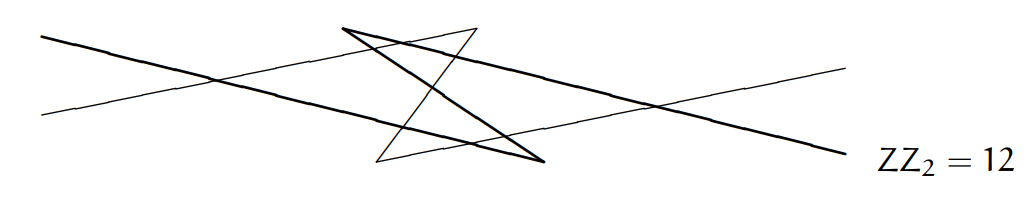
\includegraphics[width=0.7\textwidth]{images/1-13-zig-zag.PNG}
  \label{fig:example}
\end{figure}
\par

\begin{flushleft}
\textbf{Solution: }
\par
After a little thought, we realize that a zig zag is like three intersecting lines. Three intersecting line creates 7 regions. But one zig zag only creates 2 regions. So we lose 5 a region per zig zag.
We know number of regions generated by $n$ lines is, $L_n=\frac{n(n+1)}{2}+1$

So, number of regions definable by $n$ zig-zay hes is,
$$
\begin{aligned}
Z Z_n & =L_{3 n}-5 n \\
& =\frac{3 n(3 n+1)}{2}+1-5 n \\
& =\frac{9 n^2+3 n}{2}+1-5 n \\
& =\frac{9}{2} n^2+\frac{3}{2} n-5 n+1 \\
& =\frac{9}{2} n^2-\frac{7}{2} n+1
\end{aligned}
$$
\end{flushleft}

\newpage
\section{Chapter-2: Sums}

\subsection{Problem 1(2.11)}
\begin{flushleft}
\textbf{Solution: }
\par
$$
\begin{aligned}
L . H . S & =\sum_{0 \leq k<n}\left(a_{k+1}-a_k\right) b_k \\
& =\sum_{0 \leq k<n} a_{k+1} b_k-\sum_{0 \leq k<n} a_k b_k \\
& =\sum_{0 \leq k<n} a_{k+1} b_k-\sum_{1 \leq k+1 \leq n} a_{k+1} b_{k+1} -a_0b_0  + a_nb_n\\
& =\sum_{0 \leq k<n} a_{k+1} b_k-\sum_{0 \leq k \leq n-1} a_{k+1} b_{k+1}-a_0b_0 + a_nb_n \\
& =a_n b_n-a_0 b_0+\sum_{0 \leq k<n} a_{k+1} b_k-\sum_{0 \leq k<n} a_{k+1} b_{k+1}\\
& =a_n b_n-a_0 b_0-\sum_{0 \leq k<n} a_{k+1}\left(b_{k+1}-b_k\right)\\
& =R \cdot H \cdot S
\end{aligned}
$$

\end{flushleft}
\subsection{Problem 2(2.12)}
\textbf{Show that the function $p(k)=k+(-1)^k c$ is a permutation of the set of all integers; whenever $c$ is an integer.}
\par

\begin{flushleft}
\textbf{Solution: }
\par
Let,
$$
\begin{aligned}
\text { Let, } & p(k)=n \in \mathbb{N} \\
\Rightarrow & k+(-1)^k c=n \quad . . .(i) \\
\Rightarrow & k+(-1)^k c+c=n+c \\
\Rightarrow & k+\left\{(-1)^k+1\right\} c=n+c
\end{aligned}
$$
Now,
$$
\begin{aligned}
& (-1)^{k+\left\{(-1)^k+1\right\} c}=(-1)^{n+c} \\
\Rightarrow & (-1)^k \cdot (-1)^{\left\{(-1)^k+1\right\} c}=(-1)^{n+c} \\
\Rightarrow & (-1)^k \cdot (-1)^{\text {even }}=(-1)^{n+c} \\
\Rightarrow & (-1)^k=(-1)^{n+c}
\end{aligned}
$$
From (i),
$$
\begin{aligned}
& n=k+(-1)^k c \\
\Rightarrow & n=k+(-1)^{n+c} c \\
\Rightarrow & k=n-(-1)^{n+c} c
\end{aligned}
$$
So, whenever $c$ is an integer, the value of $k$ above will give $p(k)=n \in \mathbb{N}$.
Therefore, the function $p(k)=k+(-1)^k c$ is a permutation of the set of all integers; whenever $c$ is an integer.
\end{flushleft}



\newpage
\subsection{Problem 3(2.14)}
\textbf{}
\par

\begin{flushleft}
\textbf{Solution: }
\par
$\begin{aligned} 
\sum_{k=1}^n k 2^k & =\sum_{k=1}^n\left(\sum_{j=1}^k 1\right)^k \\
& =\sum_{k=1}^n \sum_{j=1}^k 2^k \\
& =\sum_{1 \leq j \leq k \leq n} 2^k \\
& =\sum_{1 \leq j \leq n} \sum_{j \leq k \leq n} 2^k \\
& =\sum_{1 \leq j \leq n}\left(\sum_{0 \leq k \leq n} 2^k-\sum_{0 \leq k \leq j-1} 2^k\right) \\
& =\sum_{1 \leq j \leq n}\left(2^{n+1} -1 -2^j + 1 \right) \\
& =\sum_{1 \leq j \leq n} 2^{n+1}-\sum_{1 \leq j \leq n} 2^j \\
& =2^{n+1} \sum_{1 \leq j \leq n} 1-\left(\sum_{0 \leq j \leq n} 2^j-1\right) \\
& =n 2^{n+1}-\left(2^{n+1}-1-1\right) \\
& =n 2^{n+1}-\left(2^{n+1}-2\right)
\end{aligned}
$
\end{flushleft}
\subsection{Problem 4(2.19)}
\textbf{Use a summation factor to solve the recurrence
$$
\begin{aligned}
T_0 & =5 \\
2 T_n & =n T_{n-1}+3 \cdot n !, \quad \text { for } n>0 .
\end{aligned}
$$}
\par

\begin{flushleft}
\textbf{Solution: }
\par
Given recurrence,
$$
\begin{aligned}
T_0 & =5 \\
2 T_n & =n T_{n-1}+3 \cdot n !
\end{aligned}
$$
Comparing with $a_n T_n=b_n T_{n-1}+c_n$, we get
$$
a_n=2, b_n=n \text { and } c_n=3 \cdot n !
$$
So, the summation factor,
$$
\begin{aligned}
s_n & =\frac{a_{n-1} a_{n-2} \cdots a_1}{b_n b_{n-1} \cdots b_2} \\
& =\frac{2 \cdot 2 \cdot \cdots 2}{n(n-1) \cdots 2} \\
& =\frac{2^{n-1}}{n !}
\end{aligned}
$$
Therefore,
$$
\begin{aligned}
T_n & =\frac{1}{s_n a_n}\left(s_1 b_1 T_0 + \sum_{k=1}^n s_k c_k\right) \\
& =\frac{1}{s_n a_n}\left(\frac{2^{1-1}}{1 !} \cdot 1 \cdot 5+\sum_{k=1}^n \frac{2^{k-1}}{k !} \cdot 3 \cdot k !\right) \\
& =\frac{1}{\frac{2^{n-1}}{n !}} \cdot 2\left(\frac{n !}{2^n}\left(5+3 \sum_{k=1}^n 2^{k-1}\right)\right. \\
& =\frac{n !}{2^n}\left(5+3\left(2^n-1\right)\right) \\
& =\frac{n !}{2^n}\left(2+3 \cdot 2^n\right) \\
& =n !\left(2^{1-n}+3\right) \quad
\end{aligned}
$$

\end{flushleft}




\subsection{Problem 5(2.20)}
\textbf{}
\par

\begin{flushleft}
\textbf{Solution: }
\par
Let $ S_n = \sum_{k=0}^{n} kH_k $
\par
Now,
% solve using perturbation method
$$
\begin{aligned}
    S_{n+1} &= \sum_{k=0}^{n+1} kH_k \\
    \Rightarrow S_{n+1} &= 0 \cdot H_0 + \sum_{k=1}^{n+1} kH_k \\
    \Rightarrow S_{n+1} &= \sum_{1 \leq k+1 \leq n+1}^{} (k+1)H_{k+1} \\
    \Rightarrow S_{n+1} &= \sum_{0 \leq k \leq n} (k+1)(H_k + \frac{1}{k+1}) \\
    \Rightarrow S_{n+1} &= \sum_{0 \leq k \leq n} (1 + kH_k + H_k) \\
    \Rightarrow S_{n+1} &= \sum_{0 \leq k \leq n} 1 + \sum_{0 \leq k \leq n} kH_k + \sum_{0 \leq k \leq n} H_k \\
    \Rightarrow S_n + (n+1)H_{n+1} &= (n+1) + S_n + \sum_{0 \leq k \leq n} H_k \\
    % find summation of H_k
    \Rightarrow \sum_{0 \leq k \leq n} H_k &= (n+1) - (n+1)H_{n+1} \\
    & = (n+1)(1-H_{n+1})  
\end{aligned}
$$
\end{flushleft}
\newpage
\subsection{Problem 6(2.21)}
\begin{flushleft}
    \textbf{Solution: }
    Let $ S_n = \sum_{k=0}^{n} (-1)^{n-k} $
    \par
    Now,
    % solve using perturbation method
    $$
        \begin{aligned}
            S_{n+1}   & = \sum_{k=0}^{n+1} (-1)^{n+1-k}  \\
            \Rightarrow \sum_{k=0}^{n} (-1)^{n+1-k} + (-1)^{n+1-(n+1)}   & = (-1)^{n+1-0} + \sum_{k=1}^{n+1} (-1)^{n+1-k}                \\
            \Rightarrow \sum_{k=0}^{n} (-1)^{n-k} \cdot (-1)^1 + (-1)^0   & = (-1)^{n+1} + \sum_{1 \leq k+1 \leq n+1}^{} (-1)^{n+1-(k+1)} \\
            \Rightarrow -S_n + 1 & = (-1)^{n+1} + \sum_{0 \leq k \leq n} (-1)^{n-k}              \\
            \Rightarrow  -S_n + 1 & = (-1)^{n+1} + S_n              \\
            \Rightarrow 2S_n & = 1 + (-1)^{n+1} \\
            \Rightarrow S_n & = \frac{1 + (-1)^{n+1}}{2} \\
        \end{aligned}
    $$

    \par

    Again let, $ T_n = \sum_{k=0}^{n} (-1)^k k $
    \par
    Now,
    % solve using perturbation method
    $$
    \begin{aligned}
        T_{n+1} &= \sum_{k=0}^{n+1} (-1)^k k \\
        \Rightarrow T_{n+1} &= (-1)^{n+1-0} \cdot 0 + \sum_{k=1}^{n+1} (-1)^{n+1-k} k \\
        \Rightarrow \sum_{k=0}^{n} (-1)^{n+1-k}k + (-1)^{n+1-(n+1)} \cdot (n+1) &= \sum_{1 \leq k+1 \leq n+1} (-1)^{n+1-(k+1)}(k+1)\\
        \Rightarrow \sum_{k=0}^{n} (-1)^{n-k} \cdot k \cdot (-1)^1 + (n+1) &= \sum_{0 \leq k \leq n} (-1)^{n-k}(k+1)\\
        \Rightarrow -T_n + (n+1) &= \sum_{0 \leq k \leq n} (-1)^{n-k}k + \sum_{0 \leq k \leq n} (-1)^{n-k} \\
        \Rightarrow -T_n + (n+1) &= T_n + S_n \\
        \Rightarrow 2T_n &= (n+1) - S_n \\
        \Rightarrow T_n &= \frac{(n+1) - S_n}{2} \\
                        &= \frac{(n+1) - \frac{1 + (-1)^{n+1}}{2}}{2} \\
                        &= \frac{2(n+1) - (1 + (-1)^{n+1})}{4} \\
                        &= \frac{2n + 2 - 1 - (-1)^{n+1}}{4} \\
                        &= \frac{2n + 1 + (-1)^{n+1}}{4} \\
    \end{aligned}
    $$

\end{flushleft}
\newpage
\subsection{Problem 7(2.23)}
\textbf{Evaluate the sum $ \sum_{k=1}^{n} (2k+1)/k(k+1)$ using partial fraction.}
\par

\begin{flushleft}
    \textbf{Solution: }
    \par
    % partial fraction using thumb rule
    Here,
    $$
        \begin{aligned}
            \frac{2k+1}{k(k+1)} & = \frac{2\cdot0 + 1}{k(0+1)} + \frac{2 \cdot (-1) + 1}{(-1)(k+1)} \\
            & = \frac{1}{k} + \frac{1}{k+1} \\
        \end{aligned}
    $$

    Now, 
    $$
    \begin{aligned}
        \sum_{k=1}^{n} \frac{2k+1}{k(k+1)} & =  \sum_{k=1}^{n} \left( \frac{1}{k} + \frac{1}{k+1} \right)  \\
        & = \sum_{k=1}^{n} \frac{1}{k} + \sum_{k=1}^{n} \frac{1}{k+1} \\
        & = H_n + \sum_{1 \leq k \leq n} \frac{1}{k+1} \\
        % replace k with k-1 in r.h.s
        & = H_n + \sum_{1 \leq k-1 \leq n} \frac{1}{(k-1)+1} \\
        % add 1 to each side of the limit of the sum
        & = H_n + \sum_{2 \leq k \leq n+1} \frac{1}{k} \\
        % make harmonic
        & = H_n +  \sum_{1 \leq k \leq n} \frac{1}{k} + \frac{1}{n+1} - \frac{1}{1}\\
        & = H_n + H_n + \frac{1}{n+1} - 1 \\
        & = 2H_n - \frac{n}{n+1} \\
    \end{aligned}
    $$

\end{flushleft}
\subsection{Problem 8(2.29)}
\textbf{Evaluate the sum $ \sum_{k=1}^{n} (-1)^k/(4k^2-1)$ using partial fraction.}
\par

\begin{flushleft}
\textbf{Solution: }
\par
Here,
$$
\begin{aligned}
    \frac{k}{4k^2-1} & = \frac{k}{(2k-1)(2k+1)} \\
    % partial fraction using thumb rule
    & = \frac{1/2}{(2k-1)(2\cdot \frac{1}{2} + 1)} + \frac{-1/2}{(2\cdot \frac{-1}{2} - 1)(2k+1)} \\
    % take 1/4 common
    & = \frac{1}{4} \left(  \frac{1}{2k-1} + \frac{1}{2k+1} \right)  \\
\end{aligned}
$$

$$
\begin{aligned}
    \sum_{k=1}^{n} \frac{(-1)^k}{4k^2-1} & = \sum_{k=1}^{n} \frac{(-1)^k}{4} \left(  \frac{1}{2k-1} + \frac{1}{2k+1} \right) \\
    & = \frac{1}{4} \left( \sum_{k=1}^{n} \frac{(-1)^k}{2k-1} + \sum_{k=1}^{n} \frac{(-1)^{k}}{2k+1} \right) \\
    % take 1st term out of the 1st fraction and last term out of the 2nd fraction
    & = \frac{1}{4} \left( \frac{(-1)^1}{2\cdot1-1} + \sum_{k=2}^{n} \frac{(-1)^k}{2k-1} +  \frac{(-1)^n}{2n+1} + \sum_{k=1}^{n-1} \frac{(-1)^{k}}{2k+1} \right) \\
    % simplify
    & = \frac{1}{4} \left( \frac{(-1)^n}{2n+1} - 1 +  \sum_{k+1=2}^{n} \frac{(-1)^{k+1}}{2k+2-1} + \sum_{k=1}^{n-1} \frac{(-1)^{k}}{2k+1} \right) \\
    & = \frac{1}{4} \left( \frac{(-1)^n}{2n+1} - 1 +  \sum_{k+1-1=2-1}^{n-1} \frac{(-1)^{k} \cdot (-1)^1}{2k+1}  + \sum_{k=1}^{n-1} \frac{(-1)^{k}}{2k+1} \right) \\
    & = \frac{1}{4} \left( \frac{(-1)^n}{2n+1} - 1 -  \sum_{k=1}^{n-1} \frac{(-1)^{k}}{2k+1}  + \sum_{k=1}^{n-1} \frac{(-1)^{k}}{2k+1} \right) \\
    & = \frac{1}{4} \left( \frac{(-1)^n}{2n+1} - 1 \right) \\
\end{aligned}
$$

\end{flushleft}

\newpage
\section{Chapter-4: Number theory}


\end{document}
